\documentclass{standalone}
\usepackage[dvipsnames, fixpdftex]{xcolor}
\usepackage{tikz}

\begin{document}
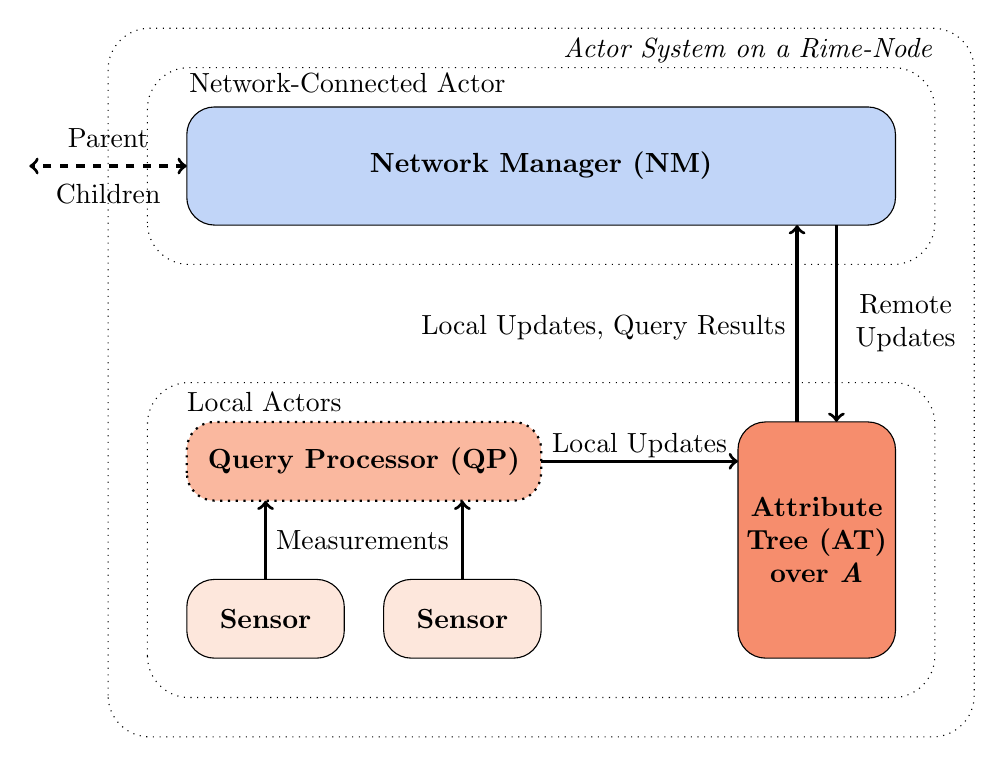
\begin{tikzpicture}
    % Reference coordinates    
    \coordinate (tA) at (7, 3.5);
    \coordinate (qprightA) at (4.5, 3.5);
    
    \coordinate (tAtop) at (8.25,4);
    \coordinate (nmtA) at (8.25,6.5);
    
    \coordinate (tAtop1) at (7.75,4);
    \coordinate (nmtA1) at (7.75,6.5);
    
    \coordinate (sens1) at (1,2);
    \coordinate (qp1) at (1,3);
    
    \coordinate (sens2) at (3.5,2);
    \coordinate (qp2) at (3.5,3);    

    \coordinate (nmOut) at (0,7.25);
    \coordinate (nmOut1) at (-2,7.25);

    % Frames
    \draw[rounded corners=15pt, dotted] (-1,0) rectangle (10,9) node[rotate=0, pos=0.5, xshift=7.5em, yshift=12em]{\textit{Actor System on a Rime-Node}};
    \draw[rounded corners=15pt, dotted] (-0.5,0.5) rectangle (9.5,4.5) node[rotate=0, pos=0.5, xshift=-10em, yshift=5em]{Local Actors};
    \draw[rounded corners=15pt, dotted] (-0.5,6) rectangle (9.5,8.5) node[rotate=0, pos=0.5, xshift=-7em, yshift=3em, align=center]{Network-Connected Actor};
    
    % Trees
    \draw[rounded corners=10pt, fill=Melon] (7,1) rectangle (9,4) node[pos=0.5, align=center]{\textbf{Attribute}  \\ \textbf{Tree (AT)} \\ \textbf{over \textit{A}}};    
   
    % Network Manager
    \draw[rounded corners=10pt, fill=CornflowerBlue!40] (0,6.5) rectangle (9,8) node[pos=0.5, align=center]{\textbf{Network Manager (NM)}};
   
    % Query processing
    \draw[rounded corners=10pt, dotted, thick, fill=Melon!60] (0,3) rectangle (4.5,4) node[pos=0.5, yshift=0em]{\textbf{Query Processor (QP)}};
   
    % Sensors
    \draw[rounded corners=10pt, fill=Melon!20] (0,1) rectangle (2,2) node[pos=0.5, yshift=0em]{\textbf{Sensor}};
    \draw[rounded corners=10pt, fill=Melon!20] (2.5,1) rectangle (4.5,2) node[pos=0.5, yshift=0em]{\textbf{Sensor}};
   
    %  sensor - qp Lines
    \draw[->, very thick](sens1) to node[pos=0.5, xshift=3.5em]{Measurements} (qp1);
    \draw[->, very thick](sens2) to (qp2);
   
    % qp - tree connecting arrows    
    \draw[->, very thick] (qprightA) to node[pos=0.5, yshift=2mm]{Local Updates} (tA);
   
    % Nm - tree connecting arrows 
    \draw[->, very thick] (nmtA) to node[pos=0.5, xshift=2.5em,yshift=0mm, align=center]{Remote \\ Updates} (tAtop);
    \draw[<-, very thick] (nmtA1) to node[pos=0.5, xshift=-7em,yshift=-0.5mm]{Local Updates, Query Results} (tAtop1);

    % Nm - outgoing
    \draw[<->, dashed, very thick] (nmOut) to node[pos=0.5, xshift=0em,yshift=1em, align=center]{Parent} node[pos=0.5, xshift=0em, yshift=-1em]{Children} (nmOut1);

\end{tikzpicture}
\end{document}